\documentclass[12pt]{article}
\usepackage[table]{xcolor}
\usepackage[shortlabels]{enumitem}
\usepackage{tabularx,xltabular}
\usepackage{graphicx}
\usepackage{hyperref}
\usepackage{verbatim}
\usepackage{geometry}
\usepackage{ulem}
\usepackage[official]{eurosym}
\usepackage{tikz}
\usetikzlibrary{arrows,backgrounds,calc,decorations.markings,patterns,3d,positioning,fit,angles, quotes}
\usepackage{pgfplots}
\pgfplotsset{compat = newest}
\usetikzlibrary{fit}
\newcommand\addvmargin[1]{
\usetikzlibrary{arrows}
\node[fit=(current bounding box),inner ysep=#1,inner xsep=0]{};}
\usepackage{cancel}
\usepackage{fontspec}
\usepackage{array}  
\geometry{a4paper, top=2cm, left=2cm, right=2cm, bottom=2cm, headsep=1cm}
\usepackage{tabu}
\usepackage{pst-node}
\usepackage{colortbl}
\usepackage{array}
\usepackage{german}
\setlength\parindent{0pt}
\newcolumntype{?}{!{\vrule width 1pt}}
\usepackage{makecell}
\renewcommand{\arraystretch}{2.5}
\usepackage{pbox}
\usepackage{amssymb}
\usepackage{amsmath}
\usepackage{booktabs}
\newcolumntype{L}[1]{>{\raggedright\let\newline\\\arraybackslash\hspace{0pt}}m{#1}}
\newcolumntype{C}[1]{>{\centering\let\newline\\\arraybackslash\hspace{0pt}}m{#1}}
\newcolumntype{R}[1]{>{\raggedleft\let\newline\\\arraybackslash\hspace{0pt}}m{#1}}
\begin{document}
\rightline{Datum: 08.12.2023}
\centerline{{\Large Üben für die Arbeit}} 
\vspace{1cm}
\noindent \\


\begin{xltabular}{\textwidth}{|C{0.75cm}|X|C{0.75cm}|X|}
\arrayrulecolor{black}\hline
a)&Setze für die Variabel x den Wert 2 ein und berechne den Wert des Terms:$$4 \cdot x + 3$$
&
b)&Setze für die Variabel b den Wert -12 ein und berechne den Wert des Terms:$$4 \cdot b + 1$$
\\\hline
c)&Vereinfache:$$3a + 2 + 3a=?$$
&
d)&Vereinfache:$$1 - 4y + 4y=?$$
\\\hline
e)&Berechne die Variable $$10\cdot b-15=5$$
&
f)&Berechne die Variable $$3\cdot b-16=11$$
\\\hline
g)&\pbox{6cm}{Bestimme den Umfang und die Fläche von: \\\tikzstyle{background grid}=[draw, black!15,step=.5cm]
\noindent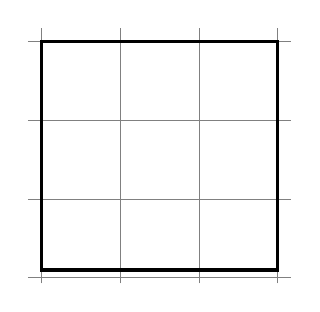
\begin{tikzpicture}[show background grid]
\draw[black, very thick] (0cm,0.1cm) rectangle (3cm,3cm);
\end{tikzpicture}}
&
h)&\pbox{5cm}{
Berechne den Flächeninhalt von:\\
\tikzstyle{background grid}=[draw, black!15,step=.5cm]
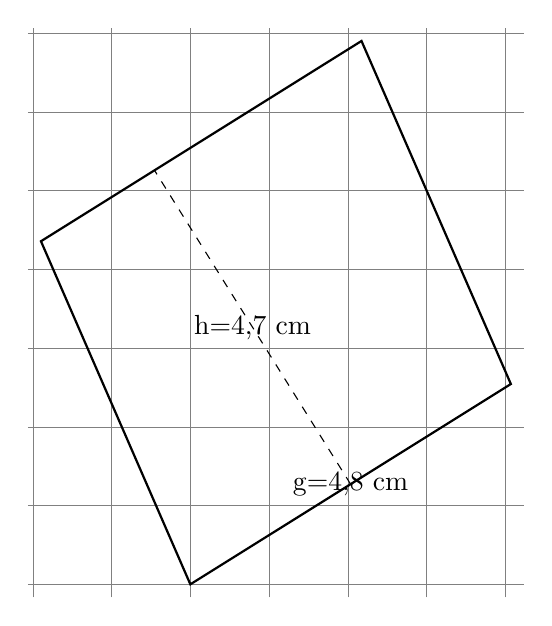
\begin{tikzpicture}[show background grid]
\draw[thick,black,rotate=32] (0,0) -- node{g=4,8 cm} ++(4.8,0) -- ++(0.7,4.7) -- ++(-4.8,0) --cycle;
\draw[dashed,black,rotate=32] (2.4,0)  -- node{h=4,7 cm} ++(0,4.7);
\end{tikzpicture}
}
\\\hline
i)&\pbox{5cm}{
Berechne den Flächeninhalt von:\\
\tikzstyle{background grid}=[draw, black!15,step=.5cm]
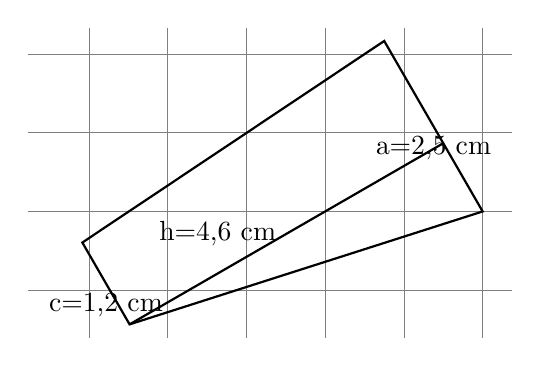
\begin{tikzpicture}[show background grid]
\draw[thick,black,rotate=120] (0,0) -- node[below]{a=2,5 cm} ++(2.5,0) -- ++(-0.3,4.6) --node[below]{c=1,2 cm} ++(-1.2,0) --cycle;
\draw[thick,black,rotate=120] (1.0,0) --node[left]{h=4,6 cm}  ++(0,4.6);
\end{tikzpicture}
}
&
j)&\pbox{5cm}{
Berechne den Flächeninhalt von:\\
\tikzstyle{background grid}=[draw, black!15,step=.5cm]
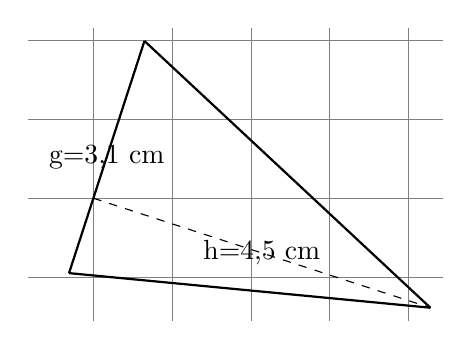
\begin{tikzpicture}[show background grid]
\draw[thick,black] (252:-2.1) -- node{g=3,1 cm} (252:1.0);
\draw[thick,black] (252:-2.1)  -- (342:4.5);
\draw[thick,black] (252:1.0)  -- (342:4.5);
\draw[dashed,black] (0,0)  -- node{h=4,5 cm} (342:4.5);
\draw[dashed,black] (0,0)  -- (252:-2.1);
\end{tikzpicture}
}
\\\hline
k)&\pbox{5cm}{
Berechne den Flächeninhalt von:\\
\tikzstyle{background grid}=[draw, black!15,step=.5cm]
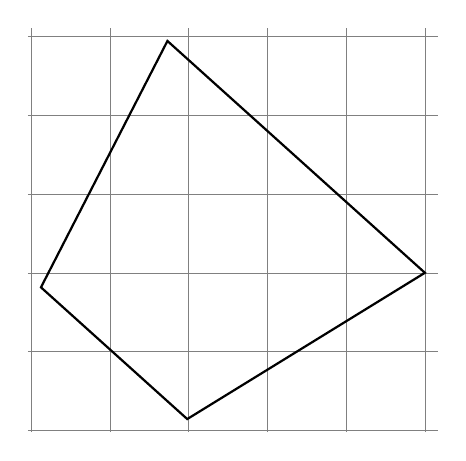
\begin{tikzpicture}[show background grid]
\draw[thick,black,rotate=138] (0,0) -- node[below]{} ++(4.4,0) -- ++(-0.9,3.4) --node[below]{} ++(-2.5,0) --cycle;
\end{tikzpicture}
}
&
l)&\pbox{5cm}{
Berechne den Flächeninhalt von:\\
\tikzstyle{background grid}=[draw, black!15,step=.5cm]
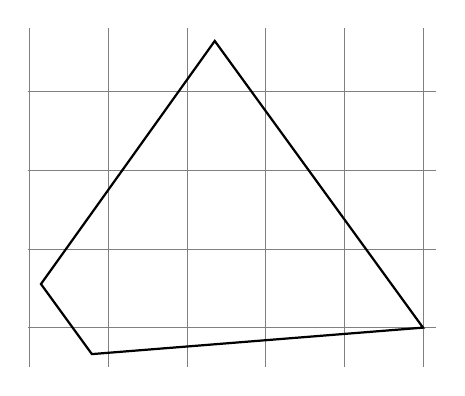
\begin{tikzpicture}[show background grid]
\draw[thick,black,rotate=126] (0,0) -- node[below]{} ++(4.5,0) -- ++(-1.2,3.6) --node[below]{} ++(-1.1,0) --cycle;
\end{tikzpicture}
}
\\\hline
m)&Stelle die Flächenformel des Rechtecks nach der fehlenden Seite um und berechne diese und den Umfang für $A=50,05~cm^2$ und $a=6,5~cm$.
&
n)&Stelle die Flächenformel des Parallelogramm nach der fehlenden Seite um und berechne diese und den Umfang für $A=34,81~cm^2$, $b=6,5~cm$ und $h_a=5,9~cm$.
\\\hline
\end{xltabular}
\vspace{0.5cm}
\newpage
\rightline{Datum: 08.12.2023}
\centerline{{\large Lösungen Üben für die Arbeit}} 
\vspace{0.5cm}

\begin{xltabular}{\textwidth}{|C{0.75cm}|X|C{0.75cm}|X|}
\arrayrulecolor{black}\hline
a)&$\begin{aligned}
\textcolor{red}{x=2} & \rightarrow\\
4 \cdot x + 3=&4 \cdot \textcolor{red}{2} + 3=11\\
\end{aligned}$
&
b)&$\begin{aligned}
\textcolor{red}{b=-12} & \rightarrow\\
4 \cdot b + 1=&4 \cdot \textcolor{red}{(-12)} + 1=-47\\
\end{aligned}$
\\\hline
c)&$3a + 2 + 3a=6a + 2$
&
d)&$1 - 4y + 4y=1$
\\\hline
e)&\begingroup\setlength{\jot}{-0.03cm}
\tikzstyle{background grid}=[draw, black!15,step=.5cm]
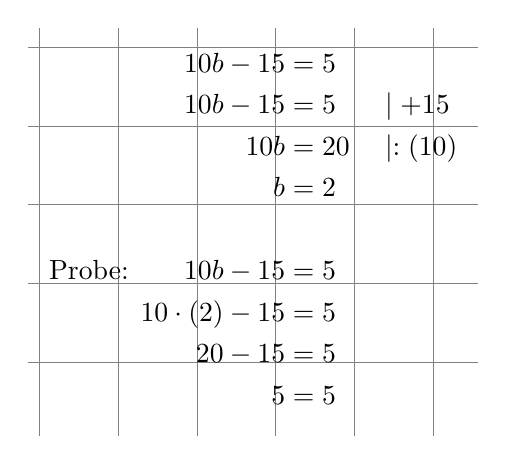
\begin{tikzpicture}[show background grid]
\node[below right] at (0,0.1) {
$\begin{aligned}
10b-15 &=5& &  \\
10b - 15 &=5& & \mid + 15\\
10b &=20& & \mid :\left(10\right)\\
b &=2& & 
\\
\\
\mbox{Probe:}\qquad 10b-15 &=5& &  \\
10\cdot \left(2\right)-15 &=5& &  \\
20-15 &=5& &  \\
5 &=5& &  \\
\end{aligned}$};
\end{tikzpicture}
\endgroup
&
f)&\begingroup\setlength{\jot}{-0.03cm}
\tikzstyle{background grid}=[draw, black!15,step=.5cm]
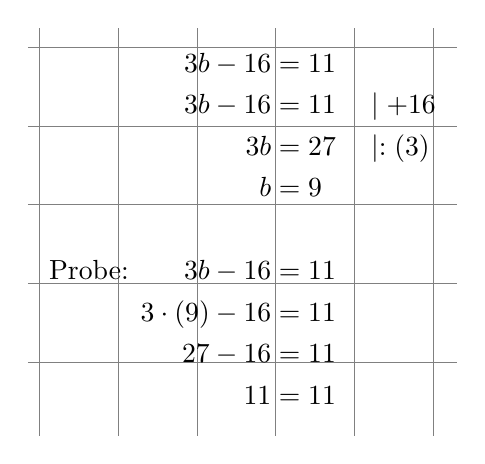
\begin{tikzpicture}[show background grid]
\node[below right] at (0,0.1) {
$\begin{aligned}
3b-16 &=11& &  \\
3b - 16 &=11& & \mid + 16\\
3b &=27& & \mid :\left(3\right)\\
b &=9& & 
\\
\\
\mbox{Probe:}\qquad 3b-16 &=11& &  \\
3\cdot \left(9\right)-16 &=11& &  \\
27-16 &=11& &  \\
11 &=11& &  \\
\end{aligned}$};
\end{tikzpicture}
\endgroup
\\\hline
g)&\pbox{6cm}{$U=2\cdot a+2\cdot b$ \\ $U=2\cdot3cm+2\cdot3cm=12cm$ \\$A=a\cdot b$ \\ $A=3\cdot3=9cm^2$ \\\tikzstyle{background grid}=[draw, black!15,step=.5cm]
\noindent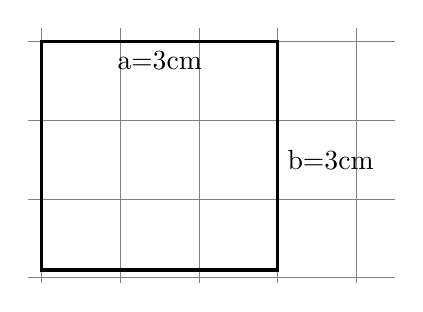
\begin{tikzpicture}[show background grid]
\draw[black, very thick] (0cm,0.1cm) rectangle (3cm,3cm);
\draw (1.5cm,3cm) node[below]{a=3cm}; 
\draw (3cm,1.5cm) node[right]{b=3cm}; 
\end{tikzpicture}}
&
h)&\pbox{5cm}{
$\begin{aligned}
geg.: g&=4,8 cm \\
   h&=4,7 cm \\
ges.: A&=? \\
A&=g\cdot h \\
&=4,8\cdot 4,7 \\
\makebox[0pt][l]{\uuline{\phantom{$A=22,56~cm^2$} } }
A&=22,56~cm^2
\end{aligned}$
\tikzstyle{background grid}=[draw, black!15,step=.5cm]
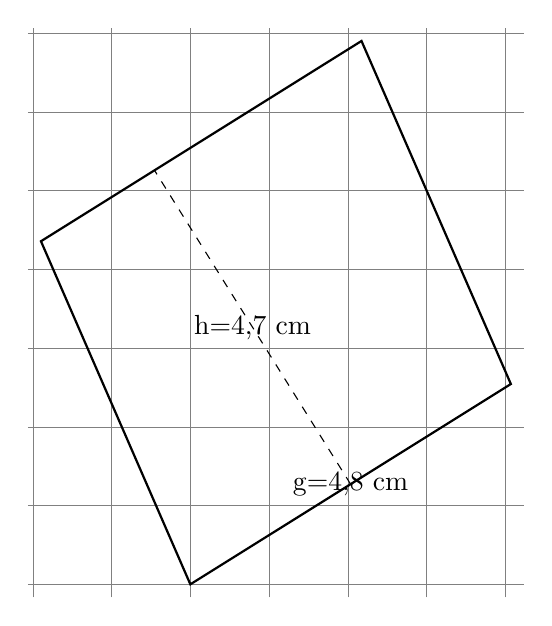
\begin{tikzpicture}[show background grid]
\draw[thick,black,rotate=32] (0,0) -- node{g=4,8 cm} ++(4.8,0) -- ++(0.7,4.7) -- ++(-4.8,0) --cycle;
\draw[dashed,black,rotate=32] (2.4,0)  -- node{h=4,7 cm} ++(0,4.7);
\end{tikzpicture}
}
\\\hline
i)&\pbox{5cm}{
\tikzstyle{background grid}=[draw, black!15,step=.5cm]
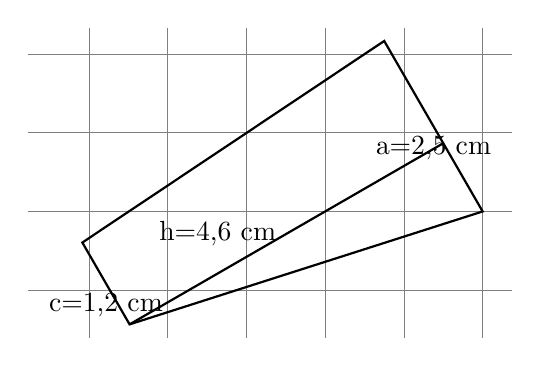
\begin{tikzpicture}[show background grid]
\draw[thick,black,rotate=120] (0,0) -- node[below]{a=2,5 cm} ++(2.5,0) -- ++(-0.3,4.6) --node[below]{c=1,2 cm} ++(-1.2,0) --cycle;
\draw[thick,black,rotate=120] (1.0,0) --node[left]{h=4,6 cm}  ++(0,4.6);
\end{tikzpicture}
$\begin{aligned}
geg.: a&=2,5 cm \\
   c&=1,2 cm \\
   h&=4,6 cm \\
ges.: A&=? \\
A&=\frac{a+c}{2}\cdot h \\
&=\frac{2,5+1,2}{2}\cdot4,6\\
\makebox[0pt][l]{\uuline{\phantom{$A=8,51~cm^2$} } }
A&=8,51~cm^2
\end{aligned}$
}
&
j)&\pbox{5cm}{
$\begin{aligned}
geg.: g&=3,1 cm \\
   h&=4,5 cm \\
ges.: A&=? \\
A&=\frac{g \cdot h}{2} \\
&=3,1 \cdot \frac{4,5}{2}\\
\makebox[0pt][l]{\uuline{\phantom{$A=6,98~cm^2$} } }
A&=6,98~cm^2
\end{aligned}$
\tikzstyle{background grid}=[draw, black!15,step=.5cm]
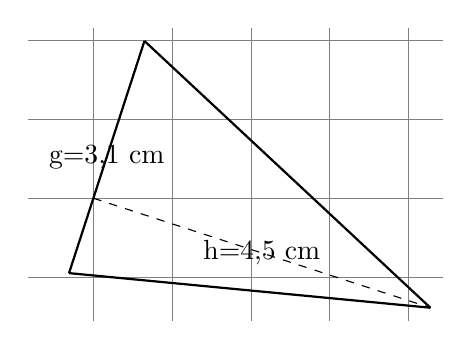
\begin{tikzpicture}[show background grid]
\draw[thick,black] (252:-2.1) -- node{g=3,1 cm} (252:1.0);
\draw[thick,black] (252:-2.1)  -- (342:4.5);
\draw[thick,black] (252:1.0)  -- (342:4.5);
\draw[dashed,black] (0,0)  -- node{h=4,5 cm} (342:4.5);
\draw[dashed,black] (0,0)  -- (252:-2.1);
\end{tikzpicture}
}
\\\hline
k)&\pbox{5cm}{
\tikzstyle{background grid}=[draw, black!15,step=.5cm]
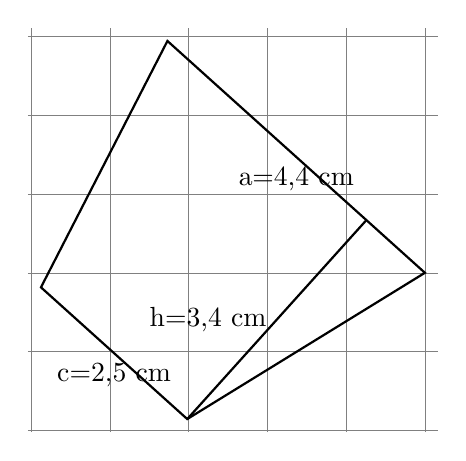
\begin{tikzpicture}[show background grid]
\draw[thick,black,rotate=138] (0,0) -- node[below]{a=4,4 cm} ++(4.4,0) -- ++(-0.9,3.4) --node[below]{c=2,5 cm} ++(-2.5,0) --cycle;
\draw[thick,black,rotate=138] (1.0000000000000004,0) --node[left]{h=3,4 cm}  ++(0,3.4);
\end{tikzpicture}
$\begin{aligned}
geg.: a&=4,4 cm \\
   c&=2,5 cm \\
   h&=3,4 cm \\
ges.: A&=? \\
A&=\frac{a+c}{2}\cdot h \\
&=\frac{4,4+2,5}{2}\cdot3,4\\
\makebox[0pt][l]{\uuline{\phantom{$A=11,73~cm^2$} } }
A&=11,73~cm^2
\end{aligned}$
}
&
l)&\pbox{5cm}{
\tikzstyle{background grid}=[draw, black!15,step=.5cm]
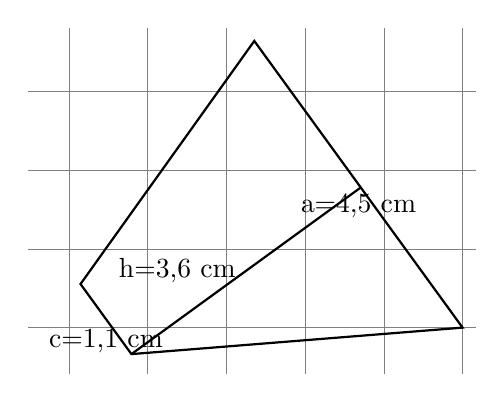
\begin{tikzpicture}[show background grid]
\draw[thick,black,rotate=126] (0,0) -- node[below]{a=4,5 cm} ++(4.5,0) -- ++(-1.2,3.6) --node[below]{c=1,1 cm} ++(-1.1,0) --cycle;
\draw[thick,black,rotate=126] (2.2,0) --node[left]{h=3,6 cm}  ++(0,3.6);
\end{tikzpicture}
$\begin{aligned}
geg.: a&=4,5 cm \\
   c&=1,1 cm \\
   h&=3,6 cm \\
ges.: A&=? \\
A&=\frac{a+c}{2}\cdot h \\
&=\frac{4,5+1,1}{2}\cdot3,6\\
\makebox[0pt][l]{\uuline{\phantom{$A=10,08~cm^2$} } }
A&=10,08~cm^2
\end{aligned}$
}
\\\hline
m)&\tikzstyle{background grid}=[draw, black!15,step=.5cm]
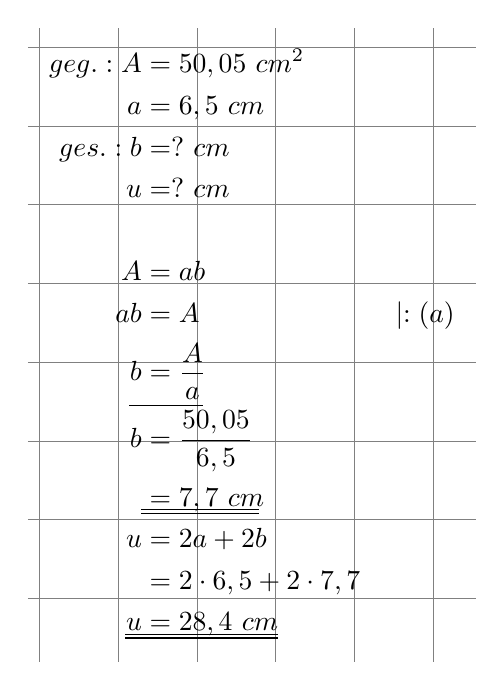
\begin{tikzpicture}[show background grid]
\node[below right] at (0,0.1) {
$\begin{aligned}
geg.: A &=50,05~cm^2& & \\
  a &=6,5~cm& & \\
ges.: b &=?~cm& & \\
u &=?~cm& & \\
& & & \\
A &=ab& & \\
ab &=A& & \mid :(a)\\
\makebox(0pt,-0.25cm)[l]{\uline{\phantom{$b ={{\frac{A}{a}}}  \\$}}}
b &={{\frac{A}{a}}}& & \\
b&=\frac{50,05}{6,5}& & \\
\makebox[0pt][l]{\uuline{\phantom{$=7,7~cm  \\$}}}
&=7,7~cm& & \\
u&=2a+2b & & \\
&=2\cdot6,5+2\cdot7,7& & \\
\makebox[0pt][l]{\uuline{\phantom{$u=28,4~cm     \\$}}}
u&=28,4~cm   & & \\
\end{aligned}$};
\end{tikzpicture}
&
n)&\tikzstyle{background grid}=[draw, black!15,step=.5cm]
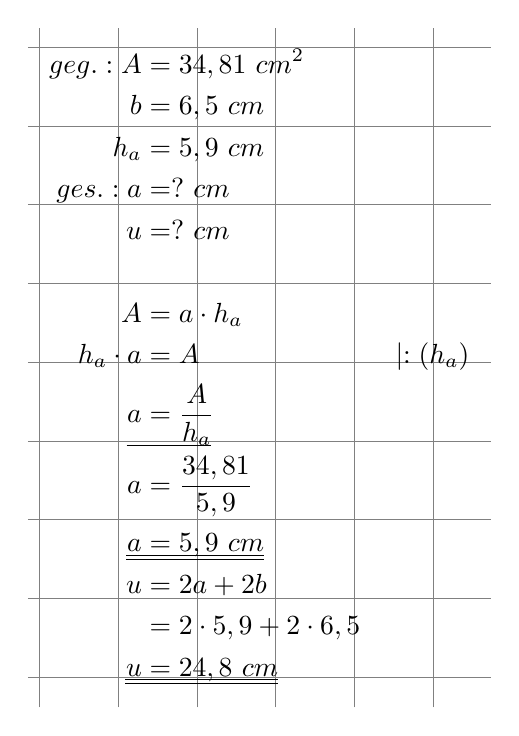
\begin{tikzpicture}[show background grid]
\node[below right] at (0,0.1) {
$\begin{aligned}
geg.: A &=34,81~cm^2& & \\
  b &=6,5~cm& & \\
  h_a &=5,9~cm& & \\
ges.: a &=?~cm& & \\
u &=?~cm& & \\
& & & \\
A &=a\cdot h_a& & \\
h_a\cdot a &=A& & \mid :(h_a)\\
\makebox(0pt,-0.25cm)[l]{\uline{\phantom{$a ={{\frac{A}{h_a}}}  \\$}}}
a &={{\frac{A}{h_a}}}& & \\
a&=\frac{34,81}{5,9}& & \\
\makebox[0pt][l]{\uuline{\phantom{$a=5,9~cm  \\$}}}
a&=5,9~cm& & \\
u&=2a+2b & & \\
&=2\cdot5,9+2\cdot6,5& & \\
\makebox[0pt][l]{\uuline{\phantom{$u=24,8~cm     \\$}}}
u&=24,8~cm   & & \\
\end{aligned}$};
\end{tikzpicture}
\\\hline
\end{xltabular}
\vspace{0.5cm}
\end{document}